\documentclass[sigconf,nonacm]{acmart}

% For images 
\usepackage{graphicx}
\usepackage{wrapfig}

\graphicspath{ {./images/} }

\begin{document}
    \title{Concurrent online sampling, for all, for free}

    \author{Daniel Brauner}
    \email{daniel.brauner@tum.de}
    
    \begin{abstract}
        This is the abstract.
    \end{abstract}

    % From the OG
    \keywords{online sampling, database statistics, query optimization}

    \maketitle

    \section{Introduction}
        % What is sampling
        A random subset of data is called a sample, usually the sample is much smaller then the actual data. In the context of Database Management Systems (DBMS) a sample is a smaller table that contains a copy of random rows from another table. The process of creating and maintaining a sample is called sampling. Maintaining hereby refers to keeping the sample up to date when the underlying data changes.
    
        % Why is sampling necessary
        Such a sample can be used by the query optimizer in modern DBMS. For instance the data stored in the sample can be used to predict the size of intermediate results when joining multiple tables. This is very important when the query optimizer tries to determine the order in which the joins should be executed. Also, the sample can be used to predict the result of aggregate queries, like SUM, COUNT, etc. 


    \section{Motivation} 
        % Current sampling algorithms
        The most naive way to provide a sample to the optimizer, would be generating it on demand. But generating a sample is not cheap, specially when the data is stored on disk. Because to create a random sample, random rows need to be read resulting in random I/O. Therefore, in some cases generating the sample can take more time then the actual query to execute.

        Some modern DBMS address this problem by only generating the sample periodically. Generating the sample still requires random I/O but the cost can be amortized over multiple queries. However, this introduces a new issues, the sample can become stale over time. Hence, predictions based on the sample can be wrong and are no longer useful for the query optimizer.

    \section{Solution}
        % What is online sampling
        Online sampling tries to address all these issues. The main idea behind online sampling is to create and maintain the sample when inserting new tuples into the database. Because every tuple that is going to be inserted is taken into consideration by the algorithm the sample is always up to date. Furthermore, no random I/O is required because no rows need to be retrieved from the disk. This approach can also be extended to support updates and deletes, but handling these operations is a little bit more involved. Modern DBMS use multiple threads for inserting and sometimes also allocate and deallocate threads on demand. Therefore, the algorithm also needs to support multithreading with a varying amount of threads.
        % Requirements
        In consequence the requirements are:
        \begin{enumerate}
            \item Keep Samples up to date while inserting new tuples
            \item As little overhead as possible, per thread and overall
            \item Use constant amount of memory
            \item Easy integration into existing solutions
            \item Minimum amount of shared memory writes (as less locks as possible)
        \end{enumerate}
        
    \subsection{Skips}
        % The idea behind skip length
        To build a random sample the algorithm needs to decide probabilistically for every inserted tuple whether the tuple is a part of the sample or not. Tuples which are inserted into the sample are called sample tuples and tuple which are not inserted are "skipped". But deciding for every tuple separately whether it is a sample tuple or not can be rather expensive. However, the amount of tuples that are skipped between two consecutive sample tuples follows a geometric distribution. Therefore, to avoid running a calculation for every inserted tuple, the length between to sample tuples can be generated randomly. This length is refereed to as the Skip length and can be used to calculate the next sample tuple. Every time a new tuple should be inserted the length can be decremented by one. If the length is equal to zero after decrementing it the current tuple is a sample tuple, otherwise it will be skipped. Once the length has reached zero a new length needs to be generated. Figure one shows an example of two Skips, 
        the white tuples are skipped and the gray tuples are sample tuples.
        \begin{figure}[h]
            \centering
            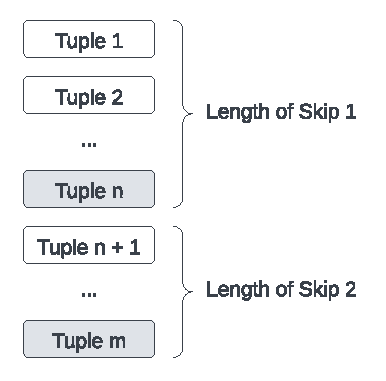
\includegraphics[height=5cm]{figure1.pdf}
            \caption{Example of two Skips with different lengths}
        \end{figure}

        % Preallocation
        The length of a Skip is stored with some additional metadata in node. To ensure the constant use of memory it is necessary that the maximum amount of threads that can be used for inserting is known when the algorithm is initialized. In consequence, all nodes can be preallocated, one for every thread and one additional node as reserve. On benefit is that no more memory allocation is required at run time and that a pointer to a node can simply be an index into the node array.

        % Multithreaded nodes
        Hence, Skips are already stored in self contained nodes, these nodes can easily be distributed among multiple threads. Once a thread has received a Skip, the thread can process tuples independently and can use its own Skip to determine which tuples to add to the sample. After the thread has reached a sample tuple and the length of the Skip has reached zero the thread needs to acquire a new Skip. Only the generation and distribution of Skips needs to be synchronized.

        % Lifecycle of a skip
        One additional field that is stored in every node, is a successor pointer. This pointer can be used to arrange nodes in a singly linked list and therefore to keep track of the state of a node. There are three states a node can be in, initially all nodes are in the free list. The free list contains all nodes that are currently not in use and can be considered as a pool of nodes that can be reused to store a Skip. If a Skip should be generated a node needs to be allocated, thus it is removed from the free list and the data of the Skip can be stored in this node. All generated Skips are stored in the list of Skips (LoS). The LoS always contains at least one Skip, this is also the reason why an extra reserve node needs to be allocated. When a thread needs to acquire a new Skip, it can pop the first item of the LoS. However, if the LoS only contains on item the thread needs to generate a new Skip and added to the LoS again. Figure two visualizes all three states and the transitions between these states.
        \begin{figure}[h]
            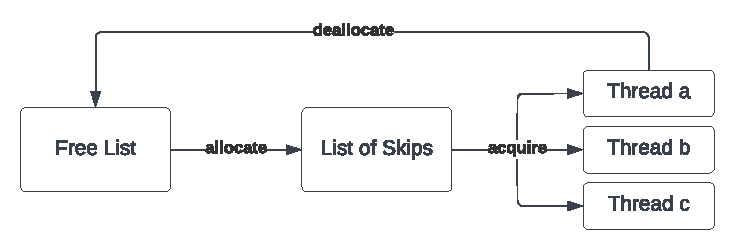
\includegraphics[height=2.8cm]{figure2.pdf}
            \caption{States of a node and the transitions between the states}
        \end{figure}

    \subsection{Inserting}
        % Description of the process
        Every thread receives an independent stream of tuples that should be inserted and therefore also sampled. The amount of tuples is unknown and each thread could stop receiving tuples at any moment. Every tuple  that the thread receives is inserted into the database and if the tuple is a sample tuple it is also added to the sample. To determine if a tuple is a sample tuple or not the thread needs to own a valid Skip. The Skip could be invalid if the length has reached zero. Therefore, if the thread currently does not own a valid Skip it needs to acquire a new one from the LoS. Once the thread owns a Skip it can use the length to determine whether the tuple is a sample tuple using the process described above.

    \section{Example}
        % An example who the algorithm works (similar to one in the OG)
        This is an example.

    \section{Evaluation}
        % Are all requirements met
        % Tables from the OG
        This is the evaluation.

\end{document}